\usetikzlibrary{graphs,graphdrawing}
\usegdlibrary{trees}

\againframe<2>{avlInsCases}

\begin{frame}[fragile,label=avlInsertCasesDiag]{AVL insert cases (revisited)}
\def\m{-}
\newcommand{\B}[1]{b: #1}
\begin{tikzpicture}
\newcommand{\mynode}{\tikzgraphnodename\\\B{\tikzgraphnodetext}}
\tikzset{
    >=Latex,
    myt/.style={binary tree layout,level distance=9mm,sibling distance=15mm,nodes={draw,circle,very thick,inner sep=0.25mm,minimum width=1.4cm,align=center,font=\small,fill=white},
        graphs/typeset=\mynode},
    inserted/.style={draw=green},
    imbalanced/.style={draw=blue,fill=blue!10},
    repChild/.style={draw=red,fill=red!10},
}
\begin{scope}[myt]
\graph {
    [name=ll] 3/\m{}2[desired at={(-3,0)},imbalanced] -> 2/\m{}1[repChild] -> 1/0[inserted]
};
\end{scope}
\begin{scope}[myt]
\graph {
    [name=rr] 1/+2[desired at={(-1,0)},imbalanced] -> 2/+1[second,repChild] -> 3/0[second,inserted]
};
\end{scope}
\begin{scope}[myt]
\graph {
    [name=lr] 3/\m{}2[desired at={(2.5,0)},imbalanced] -> 1/+1[second,repChild] -> 2/0[second,inserted]
};
\end{scope}
\begin{scope}[myt]
\graph {
    [name=rl] 1/+2[desired at={(6,0)},imbalanced] -> 3/\m{}1[second,repChild] -> 2/0[inserted]
};
\end{scope}
    \tikzset{box/.style={draw,thick}}
    \node[box,fit=(ll 1) (ll 3),label={south:single left}] (llBox) {};
    \node[box,fit=(rr 1) (rr 3),label={south:single right}] {};
    \node[box,fit=(lr 3) (lr 2) (lr 1),label={south:left-right}] {};
    \node[box,fit=(rl 3) (rl 2) (rl 1),label={south:right-left}] {};
\begin{visibleenv}<2->
\node[anchor=north west,align=left,font=\large] at ([yshift=-.75cm]llBox.south west) {
    choose rotation based on {\color{blue!70!black}lowest imbalanced node} \\
    and on {\color{red!70!black}direction of insertion} 
};
\end{visibleenv}
\end{tikzpicture}
\end{frame}

% FIXME: example with more nodes

% FIXME: get better version of this picture
\begin{frame}[fragile,label=treeRotateCases]{}
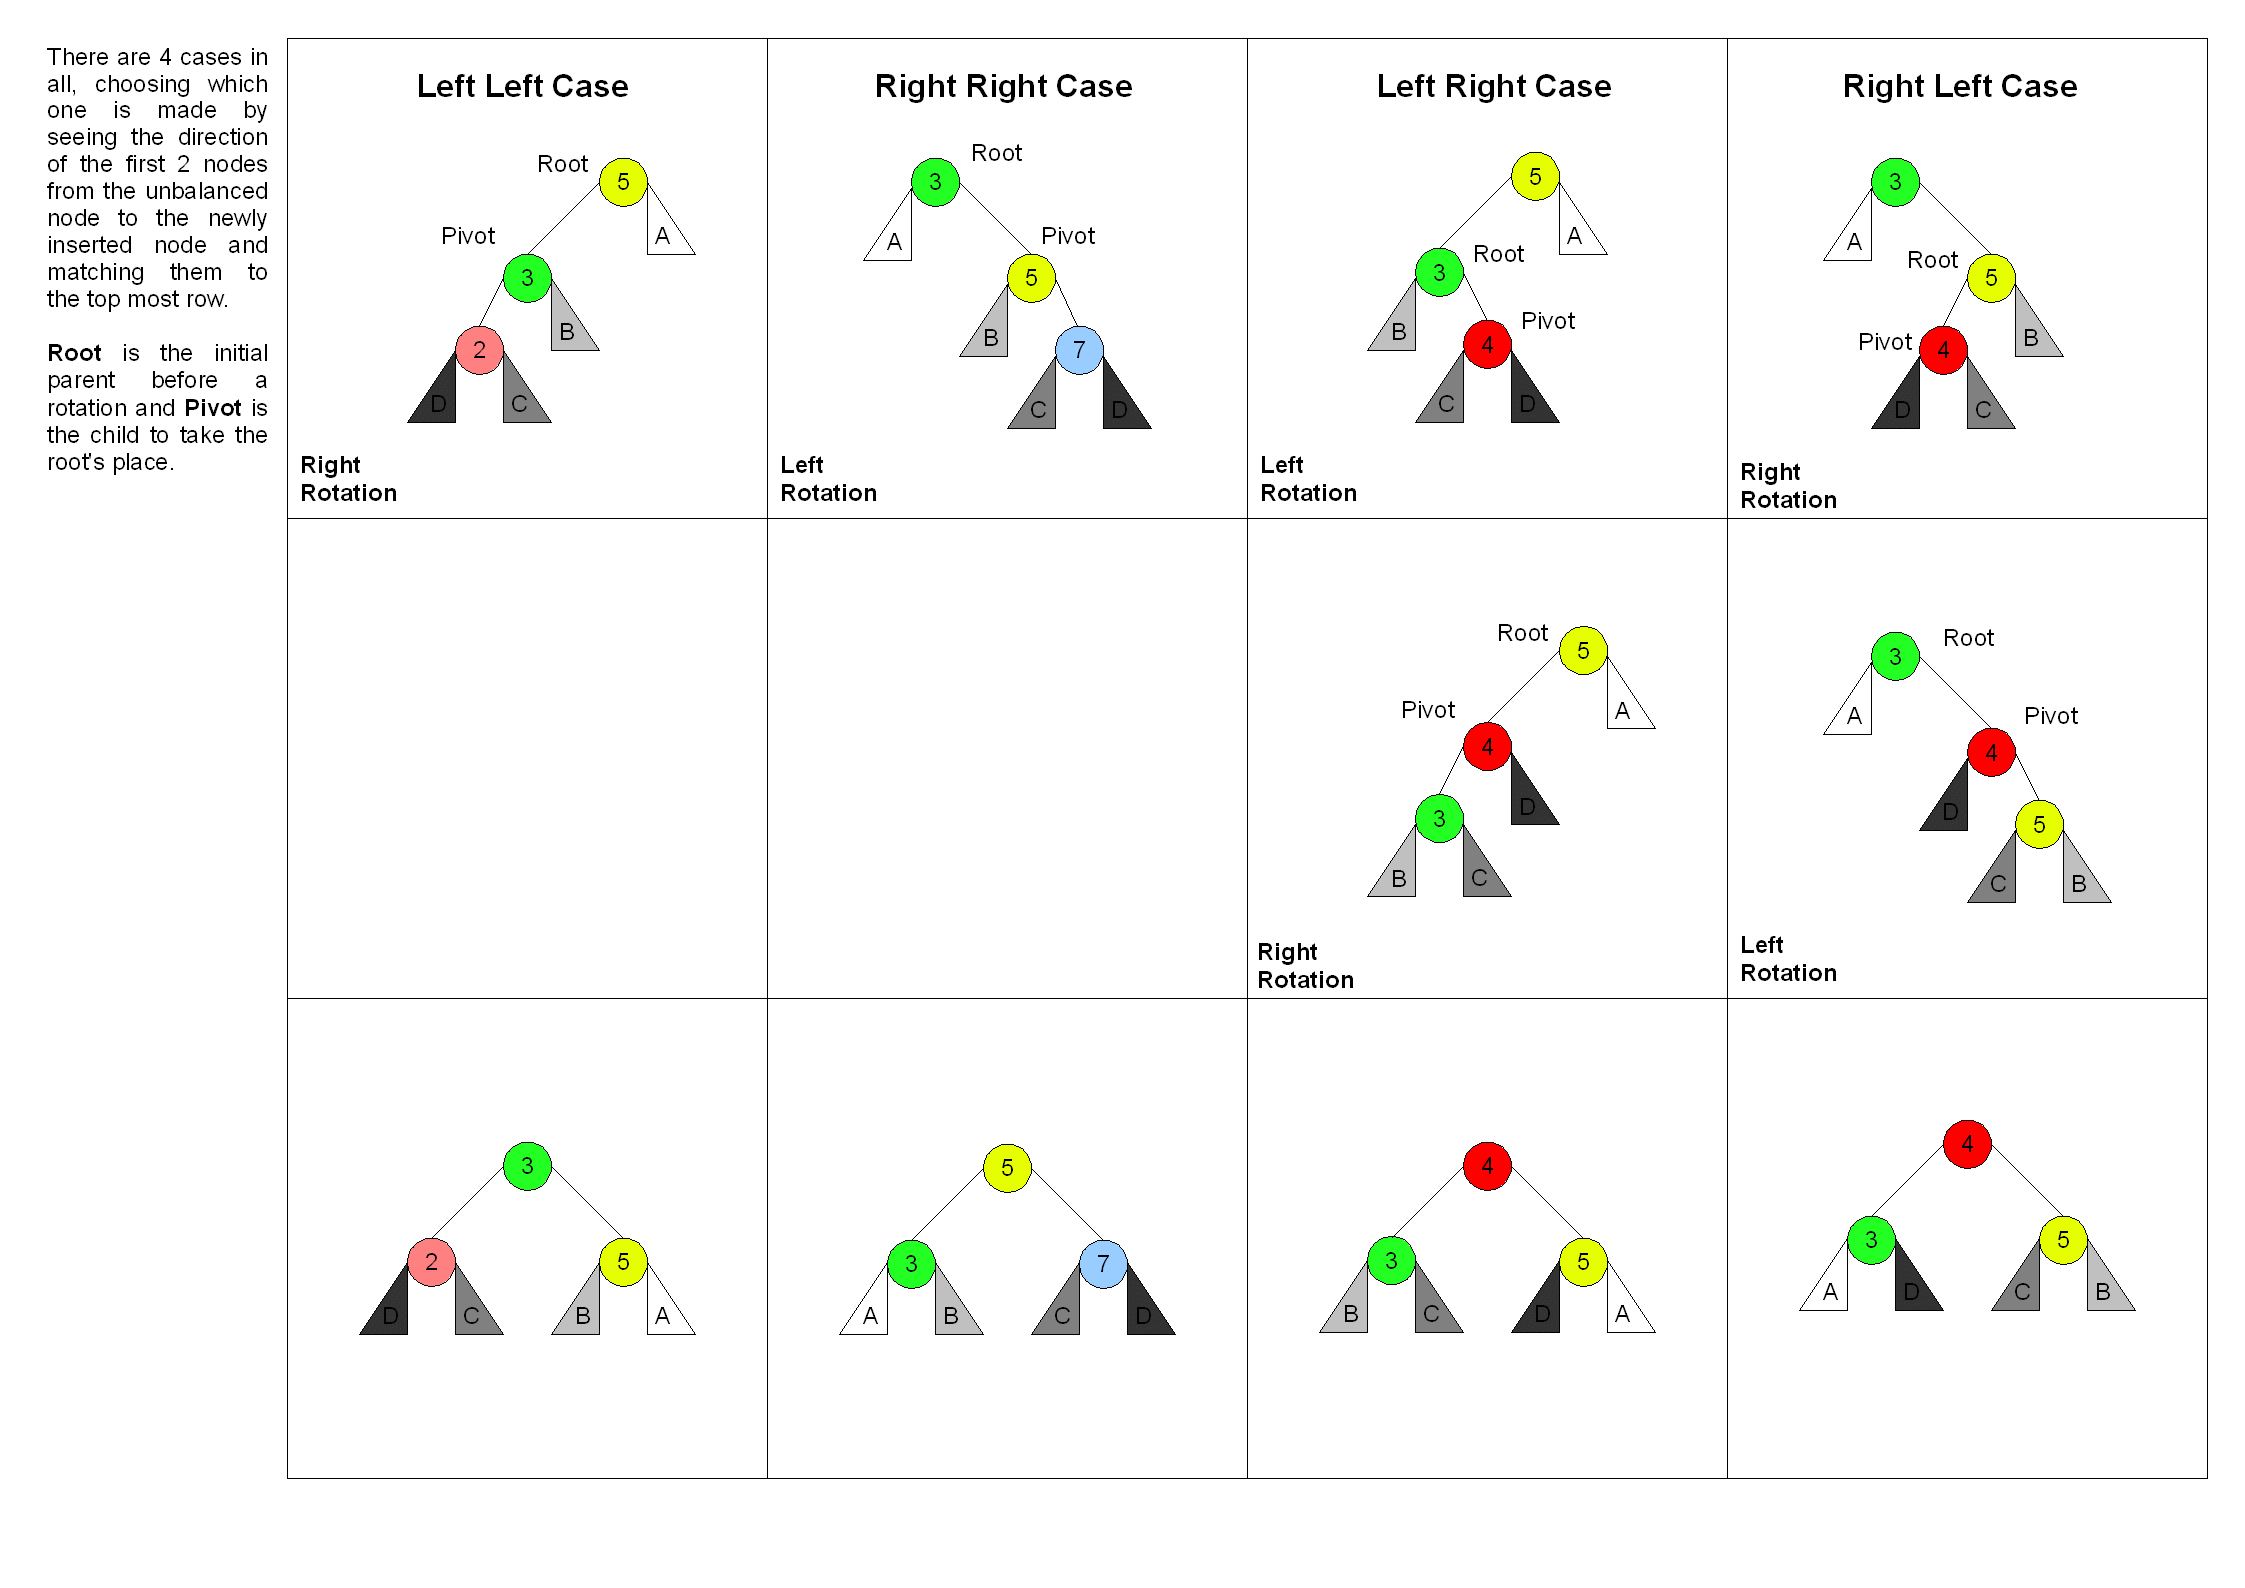
\includegraphics[height=\textheight]{Tree_Rebalancing}
\end{frame}
